% Options for packages loaded elsewhere
\PassOptionsToPackage{unicode}{hyperref}
\PassOptionsToPackage{hyphens}{url}
%
\documentclass[
]{book}
\usepackage{amsmath,amssymb}
\usepackage{iftex}
\ifPDFTeX
  \usepackage[T1]{fontenc}
  \usepackage[utf8]{inputenc}
  \usepackage{textcomp} % provide euro and other symbols
\else % if luatex or xetex
  \usepackage{unicode-math} % this also loads fontspec
  \defaultfontfeatures{Scale=MatchLowercase}
  \defaultfontfeatures[\rmfamily]{Ligatures=TeX,Scale=1}
\fi
\usepackage{lmodern}
\ifPDFTeX\else
  % xetex/luatex font selection
\fi
% Use upquote if available, for straight quotes in verbatim environments
\IfFileExists{upquote.sty}{\usepackage{upquote}}{}
\IfFileExists{microtype.sty}{% use microtype if available
  \usepackage[]{microtype}
  \UseMicrotypeSet[protrusion]{basicmath} % disable protrusion for tt fonts
}{}
\makeatletter
\@ifundefined{KOMAClassName}{% if non-KOMA class
  \IfFileExists{parskip.sty}{%
    \usepackage{parskip}
  }{% else
    \setlength{\parindent}{0pt}
    \setlength{\parskip}{6pt plus 2pt minus 1pt}}
}{% if KOMA class
  \KOMAoptions{parskip=half}}
\makeatother
\usepackage{xcolor}
\usepackage{longtable,booktabs,array}
\usepackage{calc} % for calculating minipage widths
% Correct order of tables after \paragraph or \subparagraph
\usepackage{etoolbox}
\makeatletter
\patchcmd\longtable{\par}{\if@noskipsec\mbox{}\fi\par}{}{}
\makeatother
% Allow footnotes in longtable head/foot
\IfFileExists{footnotehyper.sty}{\usepackage{footnotehyper}}{\usepackage{footnote}}
\makesavenoteenv{longtable}
\usepackage{graphicx}
\makeatletter
\def\maxwidth{\ifdim\Gin@nat@width>\linewidth\linewidth\else\Gin@nat@width\fi}
\def\maxheight{\ifdim\Gin@nat@height>\textheight\textheight\else\Gin@nat@height\fi}
\makeatother
% Scale images if necessary, so that they will not overflow the page
% margins by default, and it is still possible to overwrite the defaults
% using explicit options in \includegraphics[width, height, ...]{}
\setkeys{Gin}{width=\maxwidth,height=\maxheight,keepaspectratio}
% Set default figure placement to htbp
\makeatletter
\def\fps@figure{htbp}
\makeatother
\setlength{\emergencystretch}{3em} % prevent overfull lines
\providecommand{\tightlist}{%
  \setlength{\itemsep}{0pt}\setlength{\parskip}{0pt}}
\setcounter{secnumdepth}{5}
\usepackage{booktabs}
\ifLuaTeX
  \usepackage{selnolig}  % disable illegal ligatures
\fi
\usepackage[]{natbib}
\bibliographystyle{plainnat}
\usepackage{bookmark}
\IfFileExists{xurl.sty}{\usepackage{xurl}}{} % add URL line breaks if available
\urlstyle{same}
\hypersetup{
  pdftitle={Maple},
  pdfauthor={Ashan J},
  hidelinks,
  pdfcreator={LaTeX via pandoc}}

\title{Maple}
\author{Ashan J}
\date{2024-07-05}

\usepackage{amsthm}
\newtheorem{theorem}{Theorem}[chapter]
\newtheorem{lemma}{Lemma}[chapter]
\newtheorem{corollary}{Corollary}[chapter]
\newtheorem{proposition}{Proposition}[chapter]
\newtheorem{conjecture}{Conjecture}[chapter]
\theoremstyle{definition}
\newtheorem{definition}{Definition}[chapter]
\theoremstyle{definition}
\newtheorem{example}{Example}[chapter]
\theoremstyle{definition}
\newtheorem{exercise}{Exercise}[chapter]
\theoremstyle{definition}
\newtheorem{hypothesis}{Hypothesis}[chapter]
\theoremstyle{remark}
\newtheorem*{remark}{Remark}
\newtheorem*{solution}{Solution}
\begin{document}
\maketitle

{
\setcounter{tocdepth}{1}
\tableofcontents
}
\chapter{Matrices}\label{matrices}

There are several ways to define a matrix in Maple.
Use the help command to find the general definition of a matrix.
To work with Matrices first load the package ``\textbf{\emph{linalg}}'' Which include most linear algebra related commands.

\section{Defining matrices}\label{defining-matrices}

There are several ways to define Matrix. Let's look at them through examples.

You can use maple help.

\begin{verbatim}
> ? matrix
\end{verbatim}

\begin{verbatim}
> restart;
> with(linalg):
> M1 :=matrix (3, 3, [1,-2,-3,2,-2,2,3,-3,3]);
\end{verbatim}

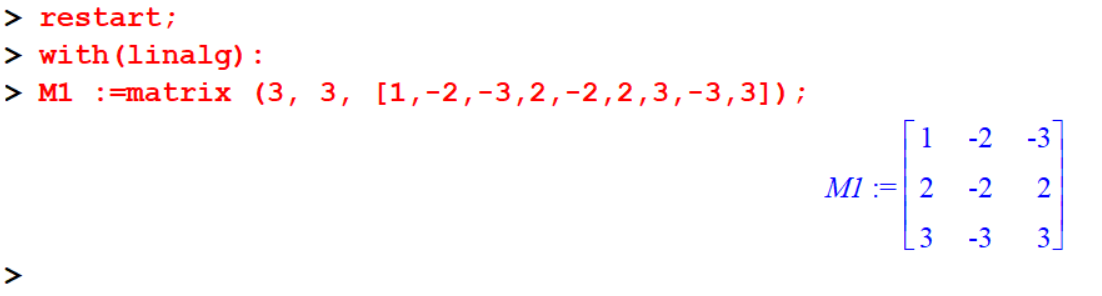
\includegraphics{figures/Lesson 4/fig1.png}

\begin{verbatim}
> M2:= matrix(3,4,[1,1/2,-1/3,1/4,2,1/2,-3/4,5/4,3,3/5,3/7,3/8]);
\end{verbatim}

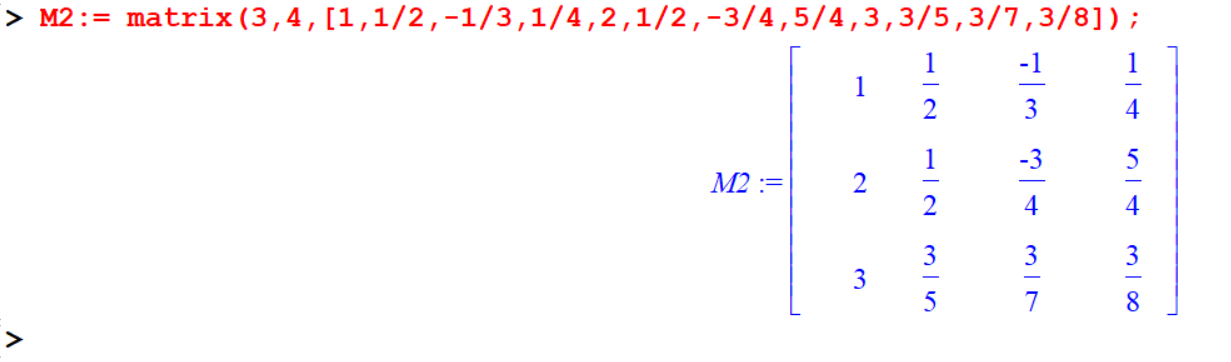
\includegraphics{figures/Lesson 4/fig2.png}

\begin{verbatim}
[> A:= matrix(3,3,[[1,-3,-2],[2,-3,5],[-4,2,6]]);
\end{verbatim}

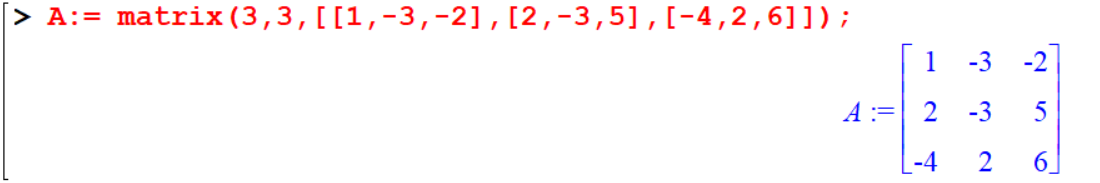
\includegraphics{figures/Lesson 4/fig3.png}

\begin{verbatim}
[> B:=matrix([[1,-3,-2],[2,-3,5],[-4,2,6]]);
\end{verbatim}

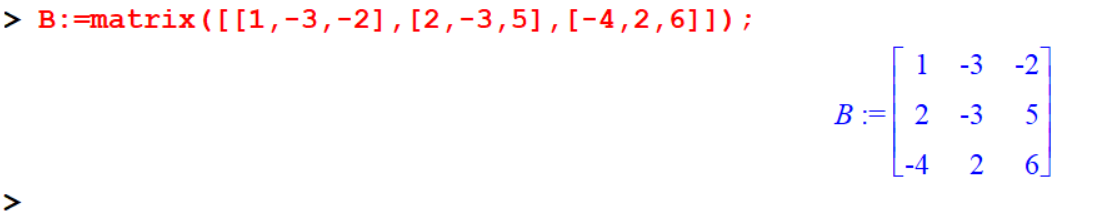
\includegraphics{figures/Lesson 4/fig4.png}

\begin{verbatim}
[> Matrix (2,2,fill=a);
\end{verbatim}

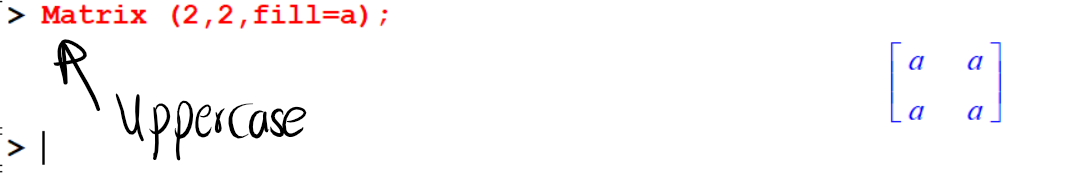
\includegraphics{figures/Lesson 4/fig5.png}

\begin{verbatim}
[> Matrix (2,2,symbol=a);
\end{verbatim}

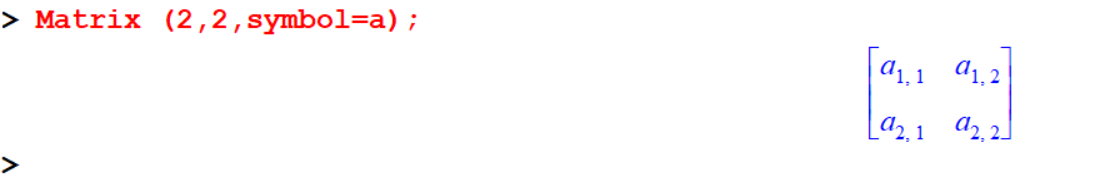
\includegraphics{figures/Lesson 4/fig6.png}

\begin{verbatim}
[> f:=i->x*i-1;
[> M:=Matrix(2,f);
\end{verbatim}

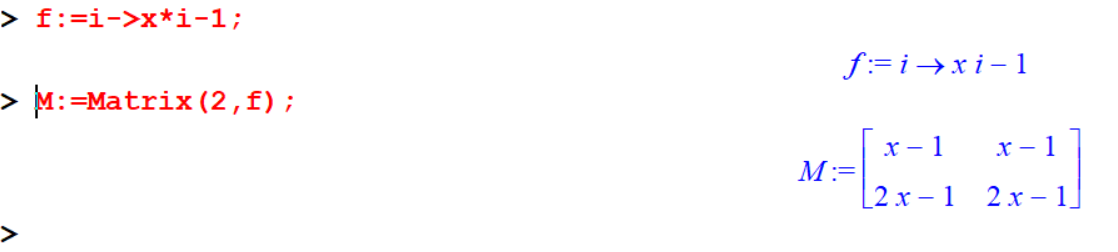
\includegraphics{figures/Lesson 4/fig7.png}

\begin{verbatim}
[> g:=(i,j)->x*(i+j—l);
[> M1:=Matrix(3,g);
\end{verbatim}

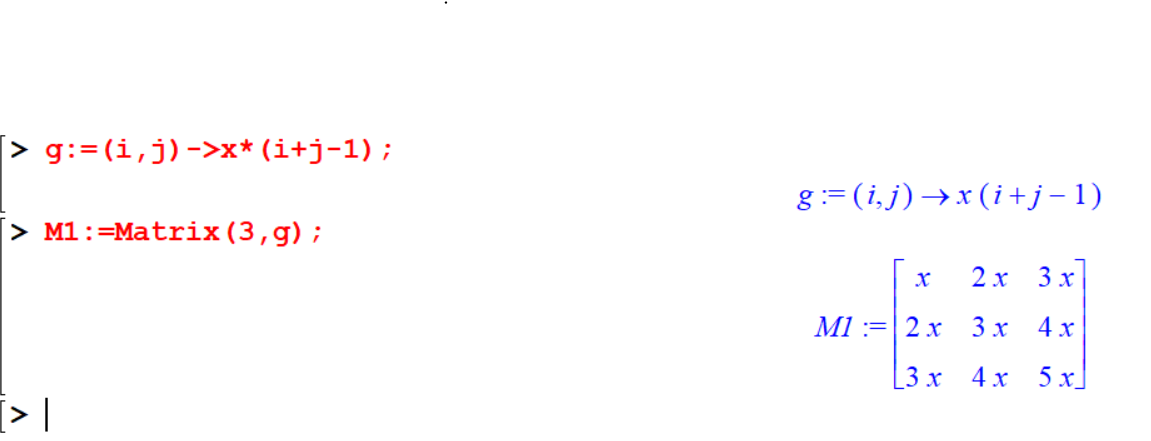
\includegraphics{figures/Lesson 4/fig8.png}
To define a diagonal matrix.

\begin{verbatim}
[> C:=diag(1,2,3);
\end{verbatim}

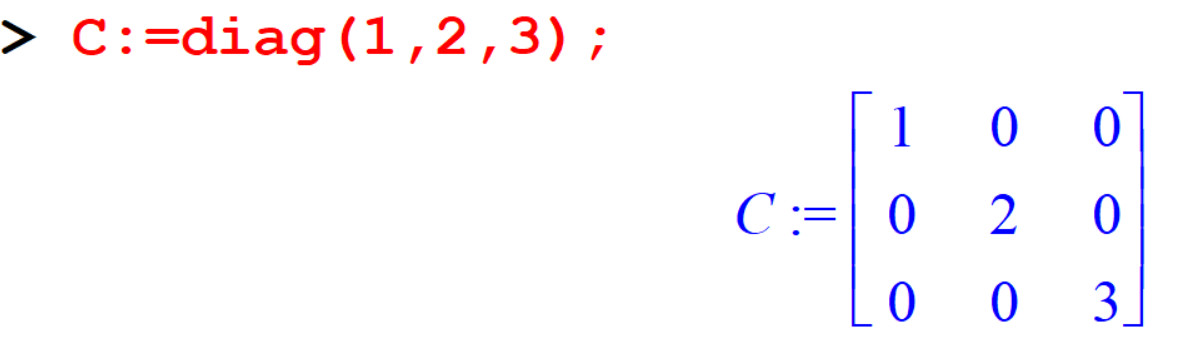
\includegraphics{figures/Lesson 4/fig16.png}

\begin{verbatim}
[> diag(1,1,1);
\end{verbatim}

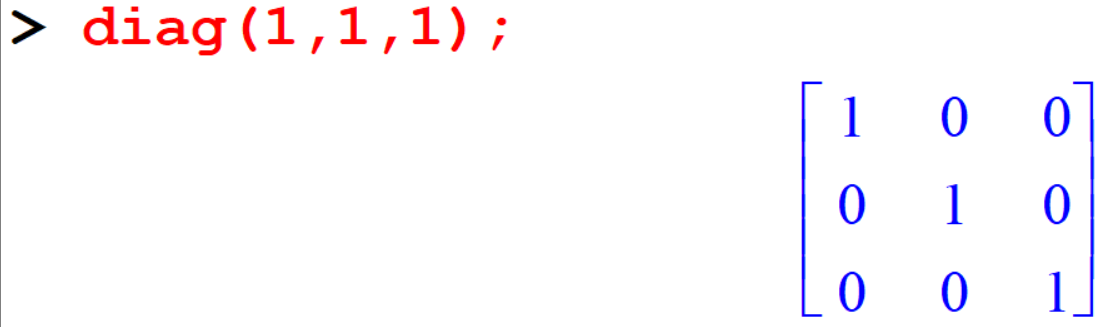
\includegraphics{figures/Lesson 4/fig17.png}

To define lower triangular matrix.

\begin{verbatim}
[> M_1:=Matrix(3,[[x],[y,y],[z,z,z]],shape=triangular[lower]);
\end{verbatim}

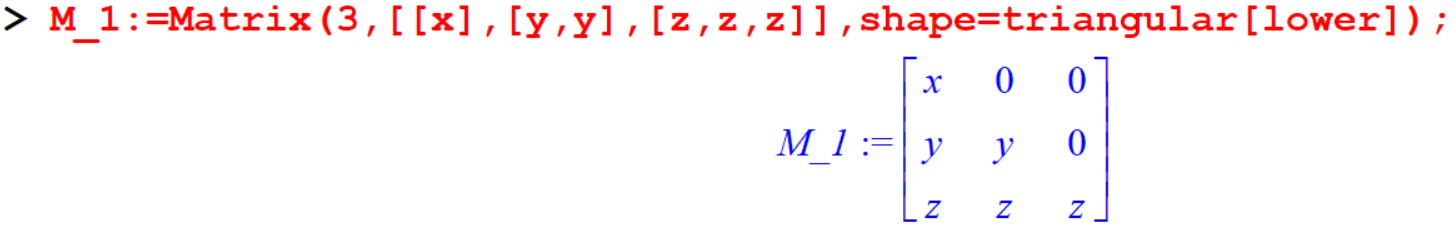
\includegraphics{figures/Lesson 4/fig18.png}

\begin{verbatim}
[> M_2:=Matrix(3,[[1,2,3],[4,5,6],[7,8,9]],shape=triangular[upper]);
\end{verbatim}

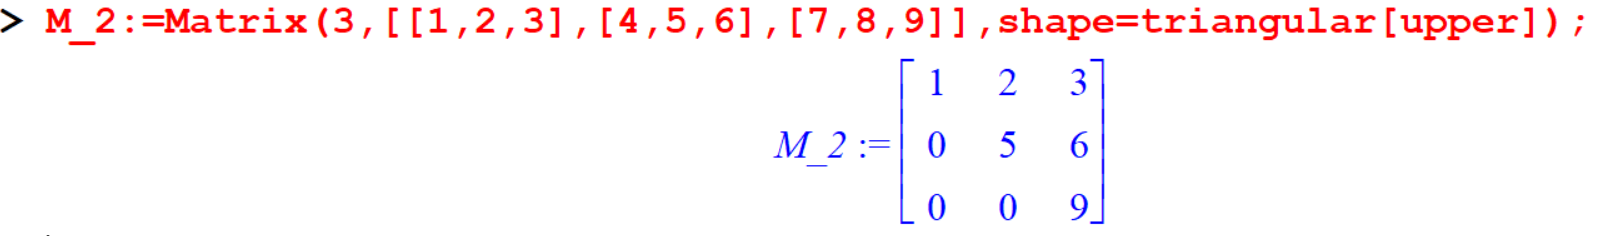
\includegraphics{figures/Lesson 4/fig19.png}

To define zero matrix

\begin{verbatim}
[> M_3:=Matrix(4,4,shape=zero);
\end{verbatim}

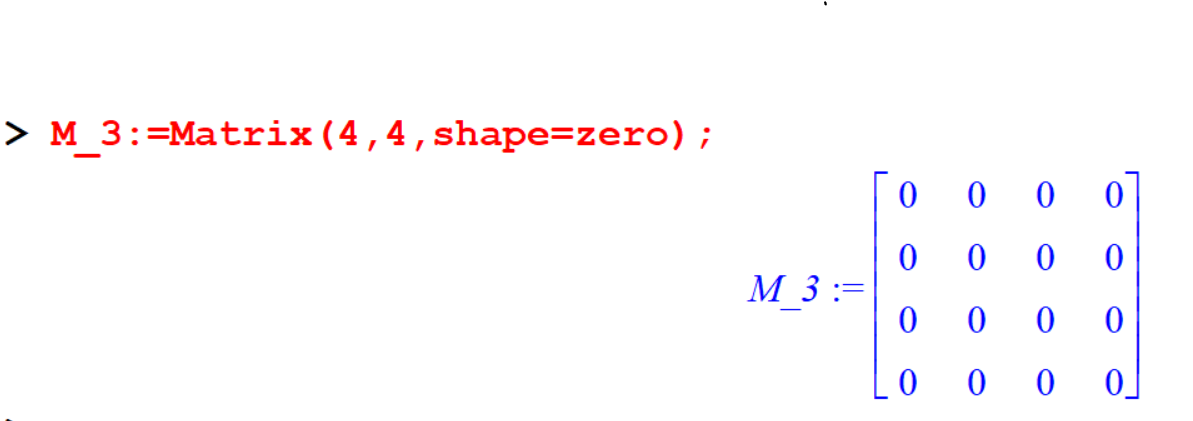
\includegraphics{figures/Lesson 4/fig20.png}

To define identity matrix

\begin{verbatim}
[> M_3:=Matrix(3,3,shape=identity);
\end{verbatim}

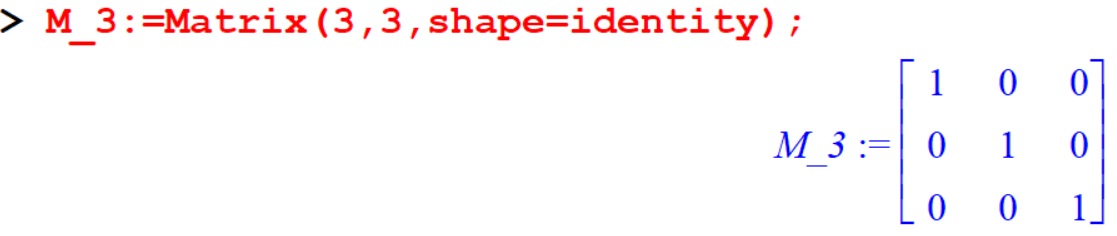
\includegraphics{figures/Lesson 4/fig21.png}

To find an entry of a matrix, follow the name of the matrix by indices inside a square bracket.

\begin{verbatim}
[> A:= matrix(3,3,[[1,-3,-2],[2,-3,5],[-4,2,6]]);
[> A[3,2];
\end{verbatim}

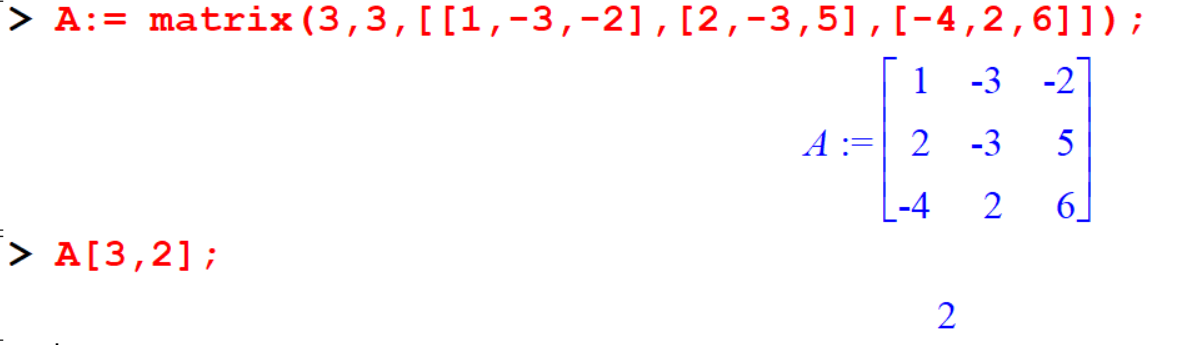
\includegraphics{figures/Lesson 4/fig22.png}

\begin{verbatim}
[> B:=matrix([[1,-3,-2],[2,-3,5],[-4,2,6]]);
[> B[1,2];
\end{verbatim}

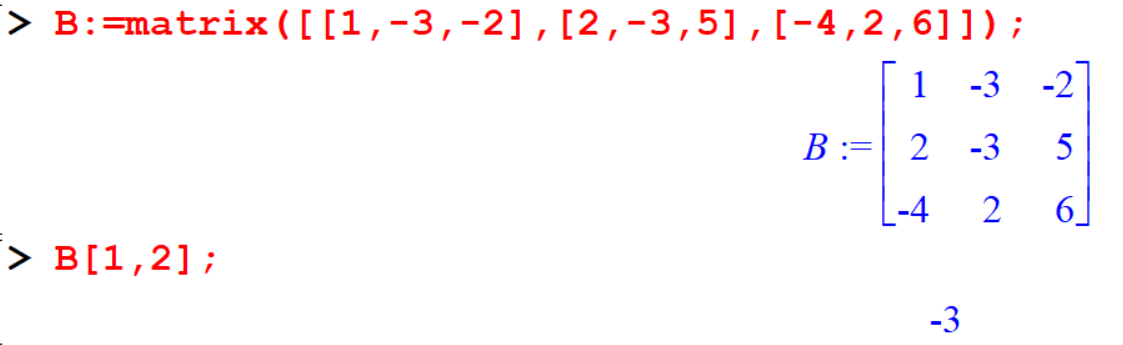
\includegraphics{figures/Lesson 4/fig23.png}
\#\# Matrix Operation

\subsection{Addition and Scalar Multiplication}\label{addition-and-scalar-multiplication}

Algebric expressions with matrices are evaluated by the command \texttt{evalm}. scalar multiplication of matrices done by the usual symbol \texttt{*}.

\begin{verbatim}
[> evalm(A+B);
\end{verbatim}

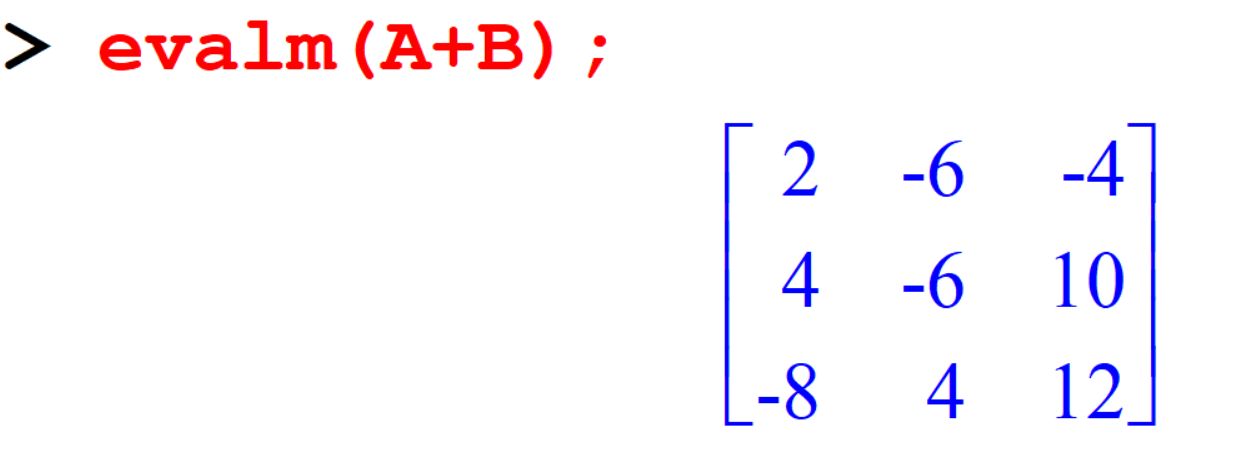
\includegraphics{figures/Lesson 4/fig24.png}

\begin{verbatim}
[> evalm(2*A+3*B);
\end{verbatim}

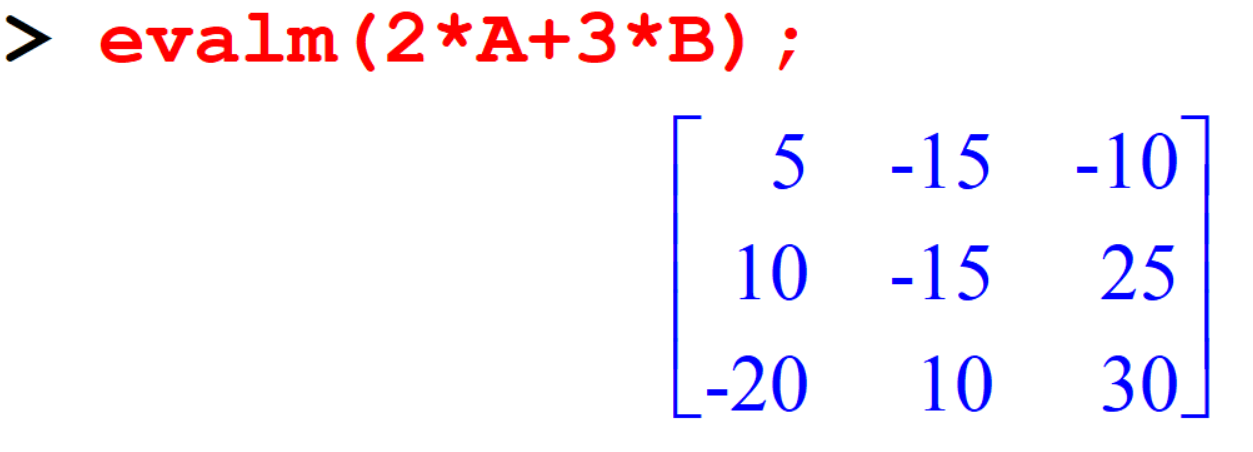
\includegraphics{figures/Lesson 4/fig25.png}

\subsection{Matrix Multiplication}\label{matrix-multiplication}

For matrix multiplication the symbol \texttt{\&*} is used.

\begin{verbatim}
[> evalm(A&*B);
\end{verbatim}

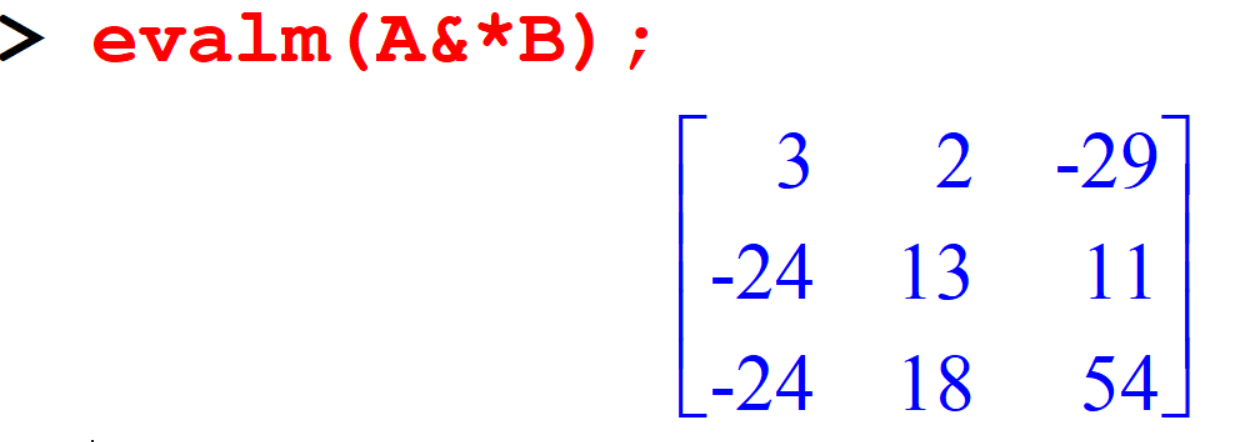
\includegraphics{figures/Lesson 4/fig26.png}

\subsection{Transpose}\label{transpose}

To get the transpose of a matrix the command \texttt{transpose} is used.

\begin{verbatim}
[> transpose(A);
\end{verbatim}

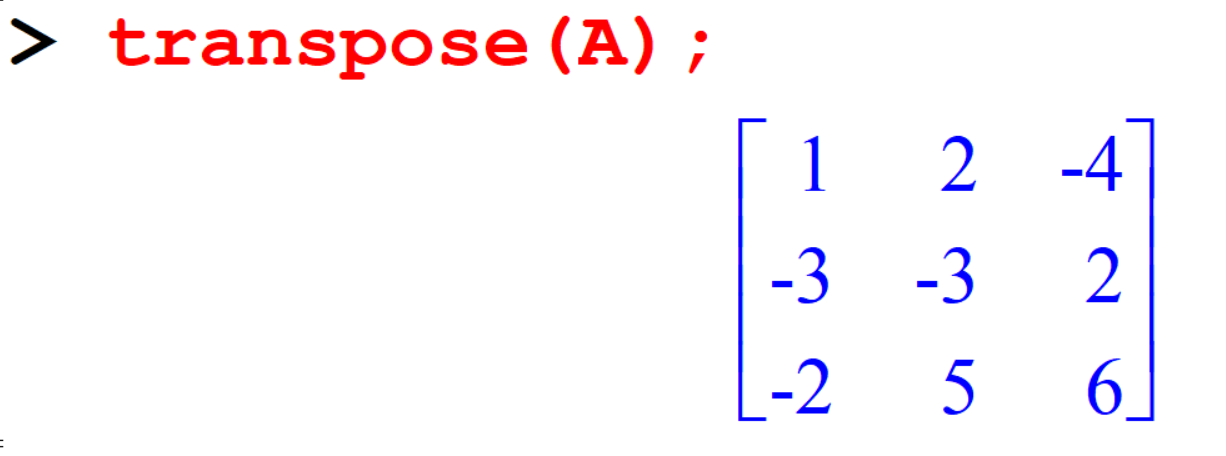
\includegraphics{figures/Lesson 4/fig27.png}

\section{Row Opreations}\label{row-opreations}

In your linear algebra class you will learn elementary row operations on matrices here we will use Maple to do the same thing.
Let's define a new matrix \(A\).

\begin{itemize}
\tightlist
\item
  \textbf{addrow(A,r1,r2,m)}\\
  Returns a copy of a matrix \(A\) in which row r2 replaced with by row(A,r2)+m*row(A,r1)
\end{itemize}

\begin{verbatim}
[> A:=matrix([[1,4,3,10],[2,1,-1,-1],[3,-1,4,11
[> addrow(A,1,2,-2);
[> addrow(%,1,3,-3);
\end{verbatim}

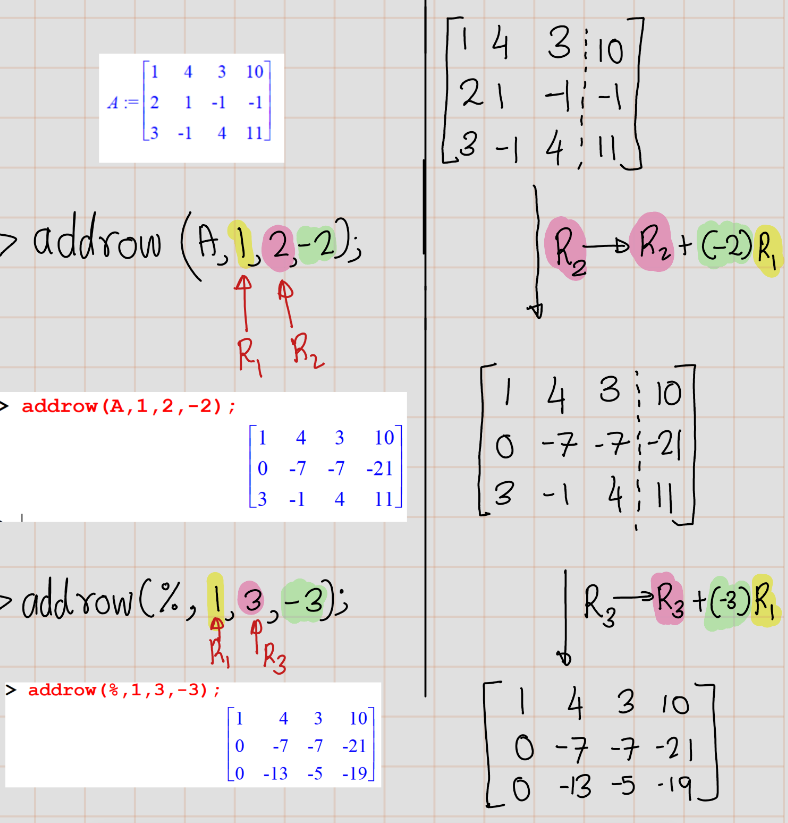
\includegraphics{figures/Lesson 4/fig9.png}

\begin{itemize}
\tightlist
\item
  \textbf{mulrow(A,row,expr)}\\
  Returns a matrix \(A\) in which has the same entries as \(A\) with the \(r^{th}\) row mutiplied by \(expr\)
\end{itemize}

\begin{verbatim}
[> mulrow(A,2,-1/7);
[> mulrow(%,3,-1/3);
\end{verbatim}

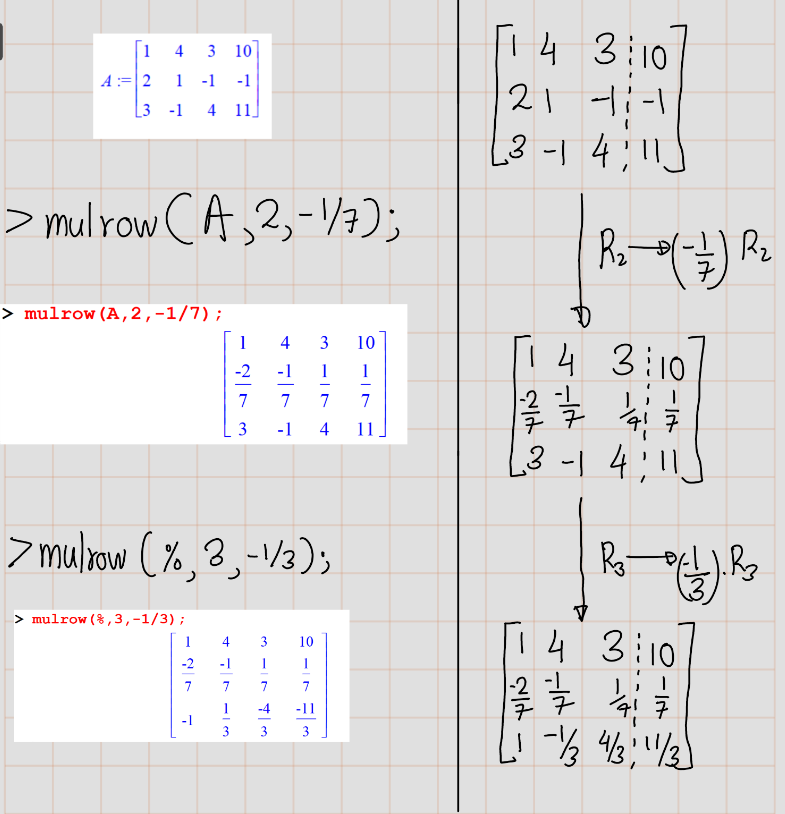
\includegraphics{figures/Lesson 4/fig10.png}

\begin{itemize}
\tightlist
\item
  \textbf{swaprow(A,r1,r2)}\\
  This command interchange row r1 and r2 of \(A\)
\end{itemize}

\begin{verbatim}
[> swaprow(A,2,3);
\end{verbatim}

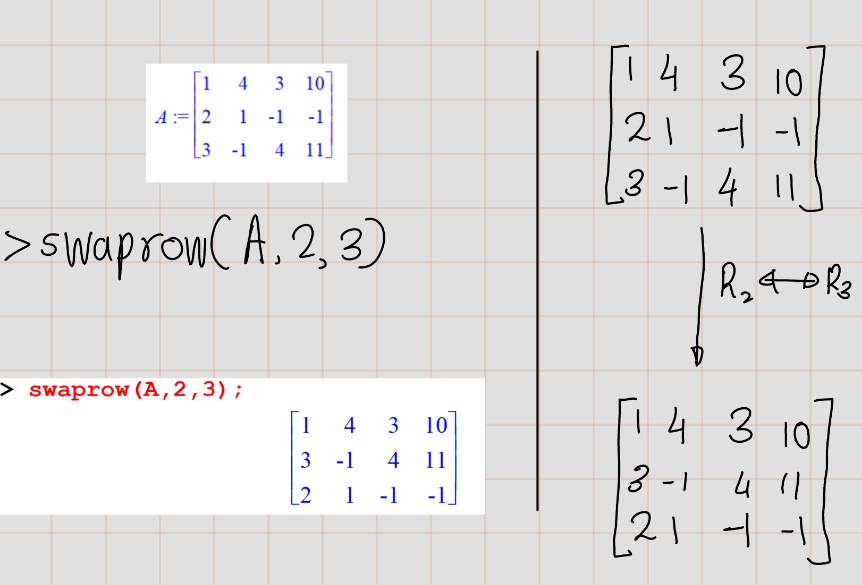
\includegraphics{figures/Lesson 4/fig11.png}

Similarly, you can learn \texttt{addcol}, \texttt{mulcol},\texttt{swapcol} commands by your self.

\section{Determinanat of Matrix}\label{determinanat-of-matrix}

To find the determinate of a matrix, maple has a special command \texttt{det}.

\begin{verbatim}
[> M1 :=matrix (3, 3, [1,-2,-3,2,-2,2,3,-3,3]);
[> det(M1);
\end{verbatim}

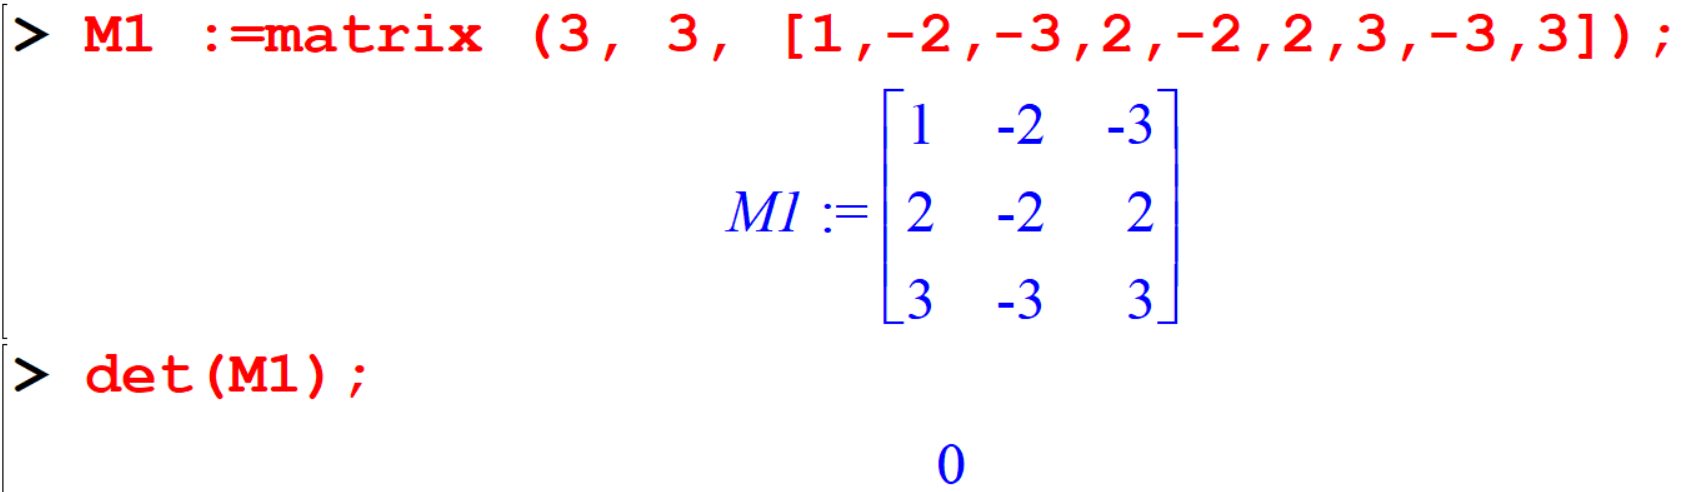
\includegraphics{figures/Lesson 4/fig12.png}

\begin{verbatim}
[> B:=matrix([[1,-3,-2],[2,-3,5],[-4,2,6]]);
[> det(B);
\end{verbatim}

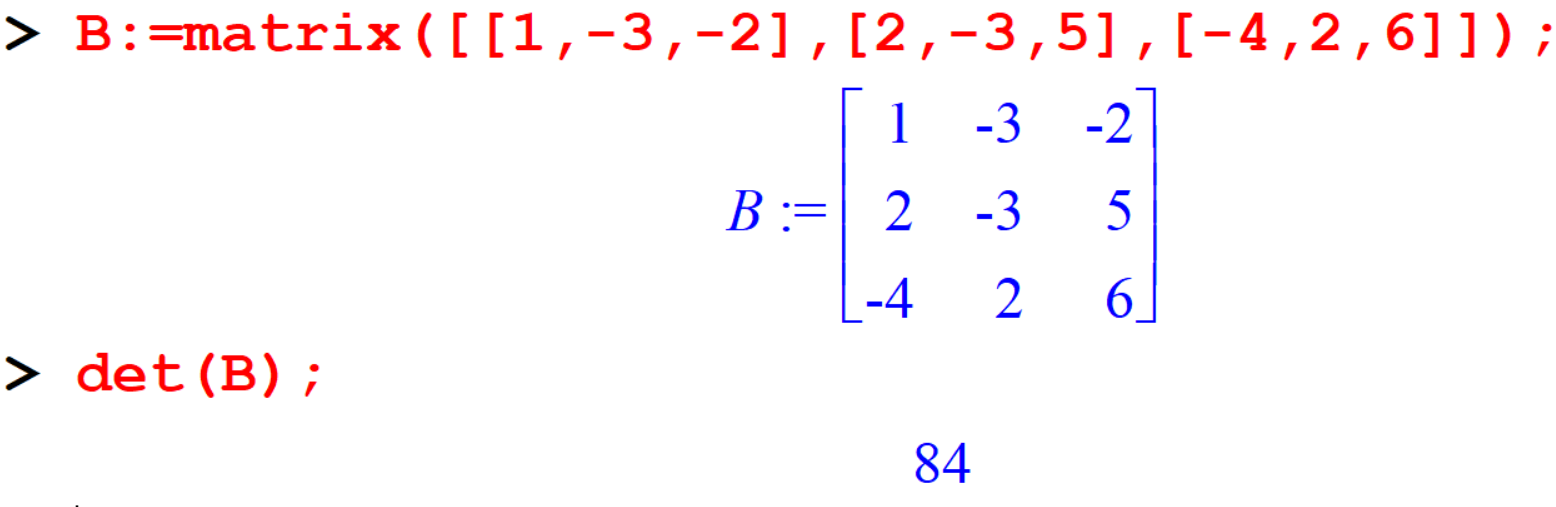
\includegraphics{figures/Lesson 4/fig13.png}

\subsection{Inverse of a matrix}\label{inverse-of-a-matrix}

The \texttt{inverse} command is used to find the inverse of a square matrix, if exists.

\begin{verbatim}
[> B:=matrix([[1,-3,-2],[2,-3,5],[-4,2,6]]);
[> inverse(B);
\end{verbatim}

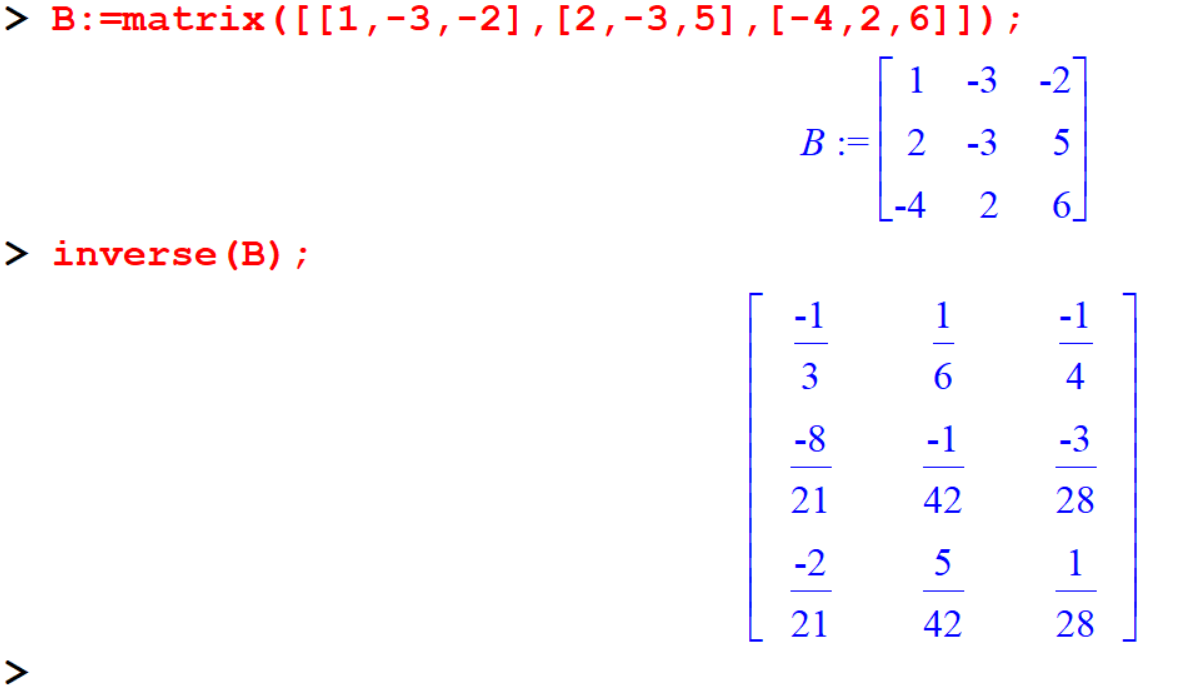
\includegraphics{figures/Lesson 4/fig14.png}

\begin{verbatim}
[> inverse([[2,-1],[3,2]]);
\end{verbatim}

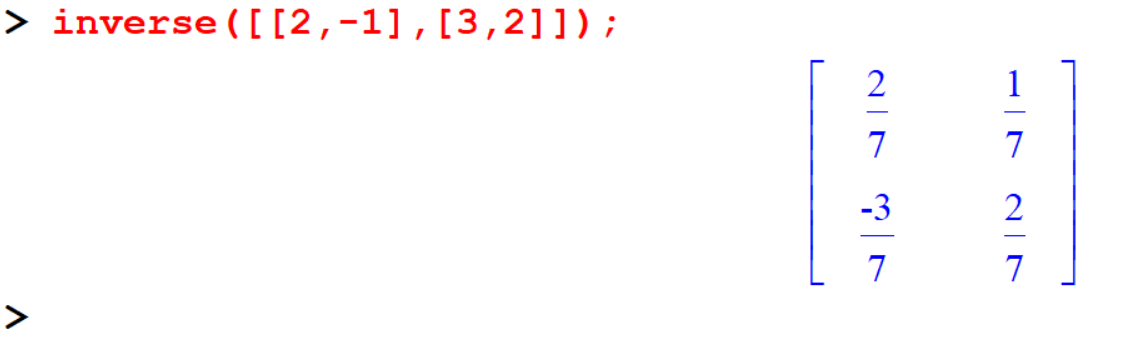
\includegraphics{figures/Lesson 4/fig15.png}

\section{Exercise}\label{exercise}

\begin{exercise}
\protect\hypertarget{exr:unnamed-chunk-1}{}\label{exr:unnamed-chunk-1}Performs the indicated computations.

A. \(\begin{bmatrix}
1 & 0 & 3 \\
2 & -1 & 6
\end{bmatrix}+
\begin{bmatrix}
2 & 0 & 4 \\
-2 & 5 & 8
\end{bmatrix}\)

B. \(5 \begin{bmatrix}
2 & 1 & 3 \\
-1 & 2 & 4 \\
-6 &1 & 5
\end{bmatrix}
-3 \begin{bmatrix}
-2 & 1 & 4 \\
5 & 0 & 7\\
2 & -1 &3
\end{bmatrix}\)

C. \(\begin{bmatrix} 2 & 3 \\ -1 & 4 \end{bmatrix}
   \begin{bmatrix} 5 & -1 \\ 2 & 7 \end{bmatrix}\)

D. \(\begin{bmatrix} 2 & 3 & 1 & 5 \\ 0 & 6 & 2 & 4 \end{bmatrix}  \begin{bmatrix} 5 & 7 & 1 \\ 2 & 0 & 3 \\ 1 & 0 & 0 \\ 0 & 5 & 6 \end{bmatrix}\)

E. \(\begin{bmatrix} 2 & 4 & 3 \\ 1 & 3 & 5 \end{bmatrix}
\begin{bmatrix} 0 & 7 & 4 \\ 2 & 3 & 0 \end{bmatrix}\)

F. \(3 \begin{bmatrix} -2 & 1 \\ 0 & 4 \\ 2 & 3 \end{bmatrix}\)

G. \(\begin{bmatrix} 1 & 0 & 3 & -1 & 5 \\ 2 & 1 & 6 & 2 & 5 \end{bmatrix} \begin{bmatrix} 7 & 1 \\ 2 & 3 \\ -1 & 0 \\ 5 & 6 \\ 2 & 3 \end{bmatrix}\)

H. \(\begin{bmatrix} 1 & -1 & 2 \\ 3 & 5 & 6 \\ 2 & 4 & -1 \end{bmatrix}
\begin{bmatrix} 2 \\ 1 \\ 3 \end{bmatrix}\)
\end{exercise}

\begin{exercise}
\protect\hypertarget{exr:unnamed-chunk-2}{}\label{exr:unnamed-chunk-2}Determine the given matrices are invertible. If they are, compute the inverse.

A. \(\begin{bmatrix} 2 & 1 \\ 3 & 2 \end{bmatrix}\)

B. \(\begin{bmatrix} 1 & 1 & 1 \\ 0 & 2 & 3 \\ 5 & 5 & 1 \end{bmatrix}\)

C. \(\begin{bmatrix} a & a \\ b & b \end{bmatrix}\)

D. \(\begin{bmatrix} 1 & 1 & 1 \\ 0 & 1 & 1 \\ 0 & 0 & 1 \end{bmatrix}\)

E. \(\begin{bmatrix} 5 & 7 & 0 \\ 2 & 1 & 3 \\ 1 & 0 & 0 \\ 0 & 4 & 3 \end{bmatrix}\)

F. \(\begin{bmatrix} 1 & 1 & 1 & 1 \\ 1 & 2 & -1 & 2 \\ 1 & -1 & 2 & 1 \\ 1 & 3 & 3 & 2 \end{bmatrix}\)

G. \(\begin{bmatrix} 1 & -3 & 0 & 2 \\ 3 & -12 & -2 & -6 \\ -2 & 10 & 2 & 5 \\ -1 & 6 & 1 & 3 \end{bmatrix}\)
\end{exercise}

\begin{exercise}
\protect\hypertarget{exr:q3}{}\label{exr:q3}Compute the \(3\times 3\) matrix whåse entries are given by the function \(y^{ij}\), Where \(i = j = 1, 2, 3\).
\end{exercise}

\begin{exercise}
\protect\hypertarget{exr:qthree}{}\label{exr:qthree}Compute the matrix,\(\begin{bmatrix}
  x & x^2 \\x^2 & x^3
  \end{bmatrix}\)
by defining a suitable function as in the exercise \ref{exr:qthree}
\end{exercise}

\begin{exercise}
\protect\hypertarget{exr:unnamed-chunk-3}{}\label{exr:unnamed-chunk-3}Which of the following matrices are skew-symmetric?
(A square matrix a symmetric if \(A^T = -A\), where \(A^T\) is the transpose of \(A\).)

A.\(\begin{bmatrix} 1 & -6 \\ 6 & 0 \end{bmatrix}\)

B.\(\begin{bmatrix} 0 & -6 \\ 6 & 0 \end{bmatrix}\)

C.\(\begin{bmatrix} 2 & -2 & 2 \\ 2 & 2 & -2 \\ 2 & 2 & 2 \end{bmatrix}\)

D.\(\begin{bmatrix} 0 & 1 & -1 \\ -1 & 0 & 2 \\ 1 & -2 & 0\end{bmatrix}\)
\end{exercise}

\begin{exercise}
\protect\hypertarget{exr:unnamed-chunk-4}{}\label{exr:unnamed-chunk-4}Convert the following matrix in to an upper triangular matrix.
\[\begin{bmatrix} 2 & 3 & -1 \\ -3 & -2 & 1 \\  0& 1 & 1\end{bmatrix}\]
\end{exercise}

\begin{exercise}
\protect\hypertarget{exr:unnamed-chunk-5}{}\label{exr:unnamed-chunk-5}Convert the following matrices into a identity matrix.

A.\(\begin{bmatrix} 2 & 7 & 3 \\ 1 & 3 & 2 \\  3 & 7 & 9\end{bmatrix}\)

B.\(\begin{bmatrix} 2 & -3 \\  3 & 4 \end{bmatrix}\)
\end{exercise}

\chapter{System of linear equations and matrices}\label{system-of-linear-equations-and-matrices}

A linear system is a collection of first degree equations. A solution to a system consists of one or more sets of specific values that our common solutions to each of the individual equations. Here is a simple example which we can solve quite easily using the solve command.
\#\# Augment of a matrix

\begin{verbatim}
[> with(linalg):
[> A:=matrix([[1,2],[2,3]]);
\end{verbatim}

\emph{Output}:

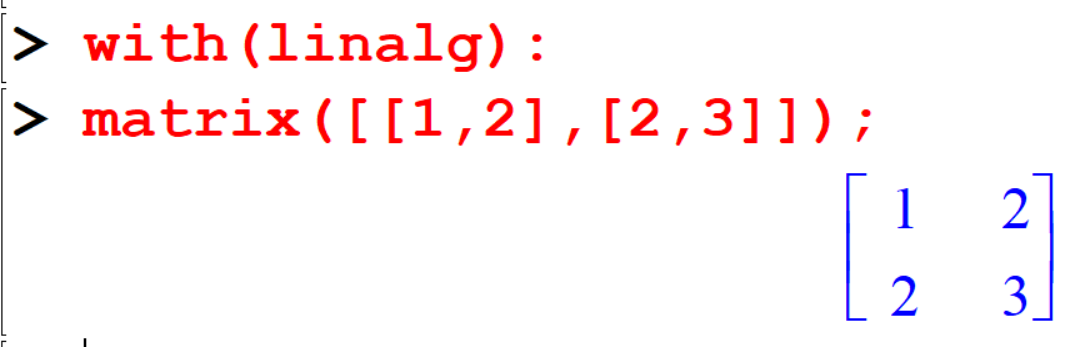
\includegraphics{figures/Lesson 5/fig1.png}

\begin{verbatim}
[> B:=matrix([[3,4,5],[6,7,8]]);
\end{verbatim}

\emph{Output}:

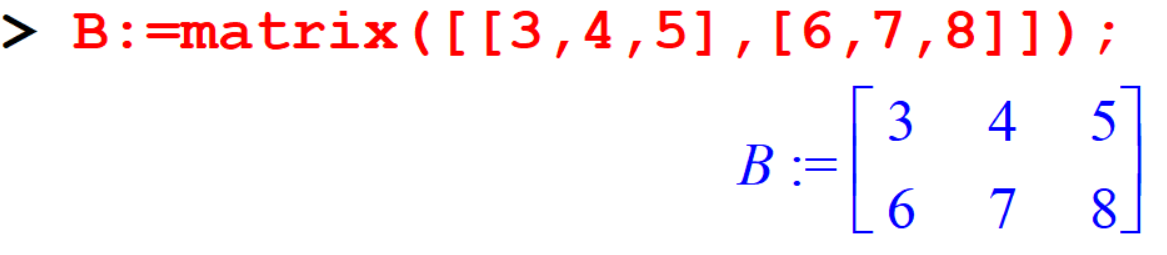
\includegraphics{figures/Lesson 5/fig2.png}

\begin{verbatim}
augment(A,B);
\end{verbatim}

\emph{Output}:

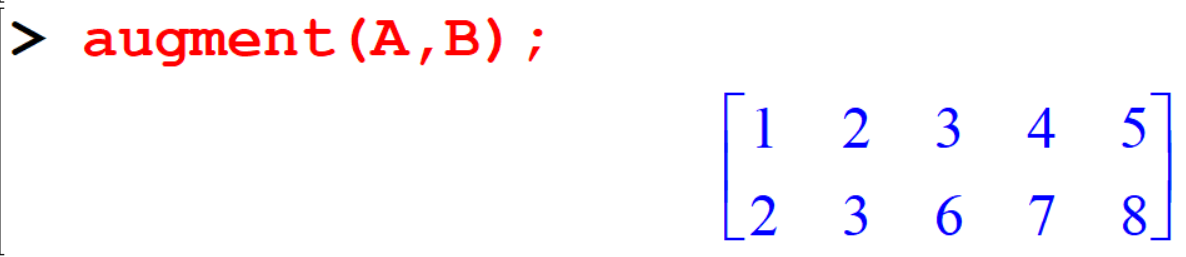
\includegraphics{figures/Lesson 5/fig3.png}

The function augment joins two or more matrices together horizontally.
The matrices and vectors must have the same number of rows.

\section{Solving Linear Systems}\label{solving-linear-systems}

\[ \begin{array}{ccccccc} 
2x &+& 5y &-& 4z &=& 9 \\
3x &+& 5y &+& 2z &=& 12 \\
4x &-& y  &+& 5z &=& -3 
\end{array} \]

\[
\underbrace{\begin{bmatrix}
2 & 5 & -4 \\
3 & 5 & 2   \\
4 & -1 & 5  
\end{bmatrix}}_A
\underbrace{\begin{bmatrix}
x \\ y\\z
\end{bmatrix}}_X
=
\underbrace{\begin{bmatrix}
9\\12\\-3
\end{bmatrix}}_B
\]

\subsection{Method I}\label{method-i}

A linear system is a collection of first degree equations.
A solution to a system consists of one or more set of specific values that our common solution to each of the individual equations.
Here is a simple example which we can solve quite easily using the solve command.

\begin{verbatim}
[> sys:={2*x+5*y-4*z=9,3*x+5*y+2*z=12,4*x-y+5*z=-3};
[> solve(sys,{x,y,z});
\end{verbatim}

\emph{Output}:

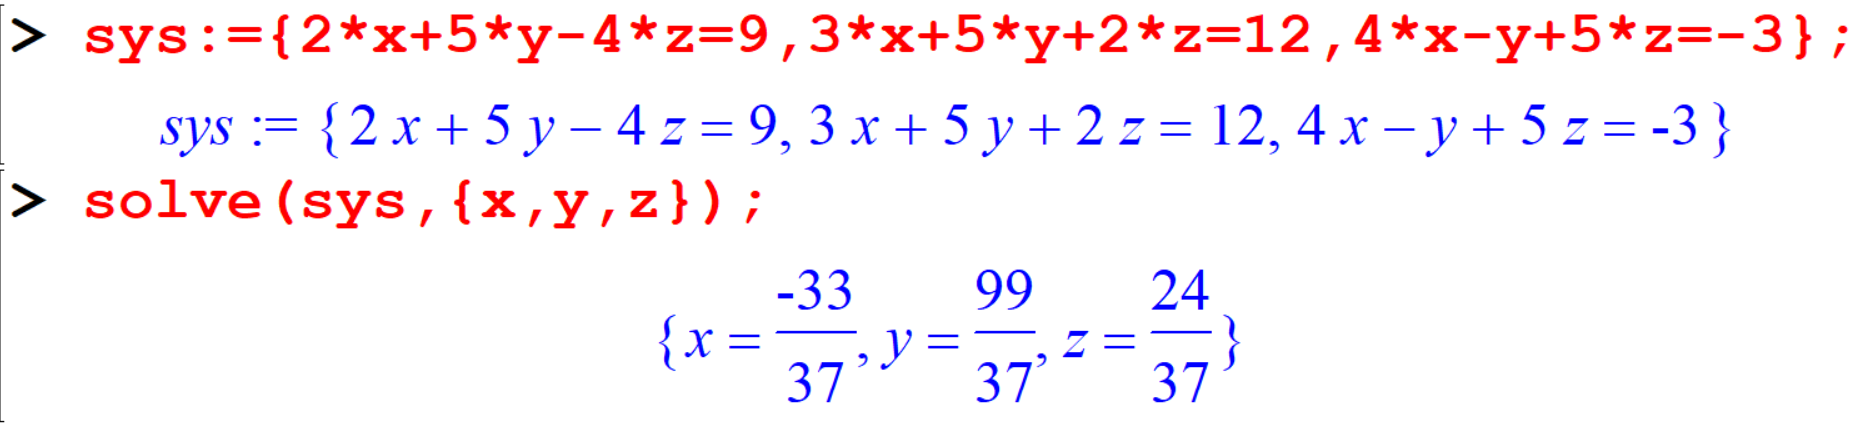
\includegraphics{figures/Lesson 5/fig4.png}

Maple will automatically use fractions, however you can force decimal answers using the \textbf{\emph{evalf}} command.

\begin{verbatim}
[> evalf(%);
\end{verbatim}

\emph{Output}:

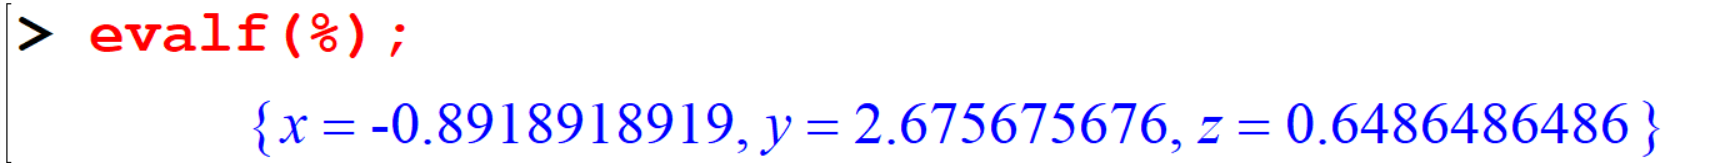
\includegraphics{figures/Lesson 5/fig5.png}

\subsection{Method II}\label{method-ii}

We can also convert the above system of equations to a matrix system.

\begin{verbatim}
[> A:=genmatrix(sys,[x,y,z],b);
[> evalm(b);
\end{verbatim}

\emph{Output}:

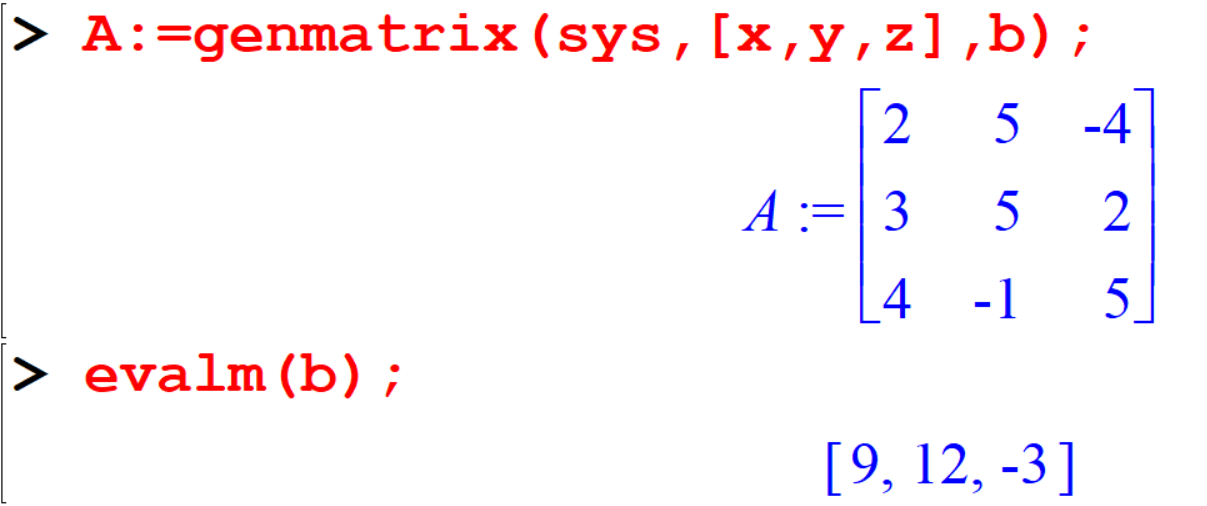
\includegraphics{figures/Lesson 5/fig6.png}

In this case ,

\begin{itemize}
\tightlist
\item
  \(A\) is the coefficient matrix, and
\item
  \(b\) is vector representing the constant values.
\end{itemize}

The command \texttt{evalm(b)} evaluated \(b\) as a matrix (a vector is a \(n \times 1\) matrix).
In other words, this command simply writes out what the vector \(b\) looks like.

\begin{verbatim}
[> linsolve(A,b);
\end{verbatim}

\emph{Output}:

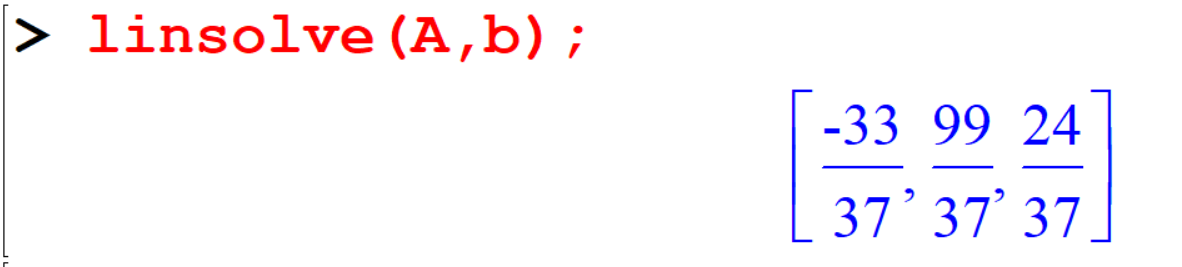
\includegraphics{figures/Lesson 5/fig7.png}

\subsection{Method III}\label{method-iii}

Another way to solve a matrix equation \(Ax = b\) is to left multiply both sides by the inverse matrix \(A^{-1}\), if it exists, to get the solution \(x = A^{-1}b\).

\begin{verbatim}
[>  inverse(A);
[> evalm(inverse(A)&*b);
\end{verbatim}

\emph{Output}:

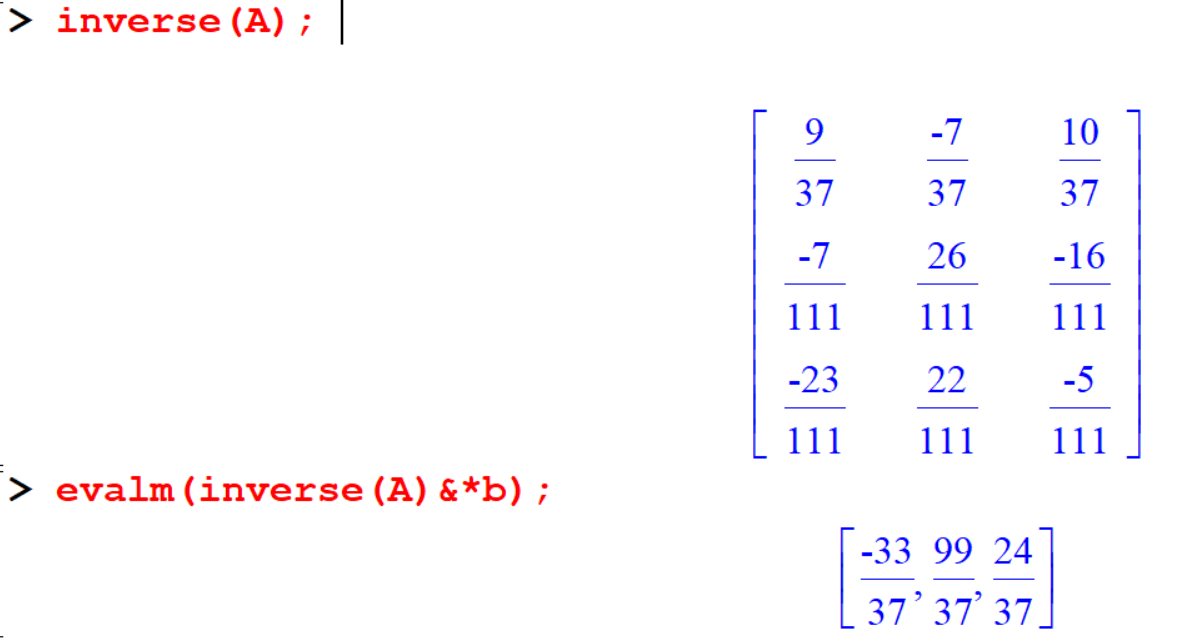
\includegraphics{figures/Lesson 5/fig8.png}

The \texttt{evalm} command forces a matrix computation and express the result.

\begin{center}\rule{0.5\linewidth}{0.5pt}\end{center}

\section{Dependent Systems:}\label{dependent-systems}

Some systems are dependent which means there are an infinite number of solutions. The form of these solutions will entail the use of parameters.
Let's look an example using two different methods; \texttt{solve} and \texttt{linsolve}.

\begin{example}
\protect\hypertarget{exm:unnamed-chunk-6}{}\label{exm:unnamed-chunk-6}\[
\begin{array}{ccccccccc}
x &-& 2y&+& z &=& &3\\
x &+& y &-& 2z&=&-&4\\
2x&-& y &-& z &=&-&1  
\end{array}
\]
\end{example}

\begin{verbatim}
[> restart;
[> with(linalg):
[> sys:={x-2*y+z=3,x+y-2*z=-4,2*x-y-z=-1};
[> solve(sys,{x,y,z});
\end{verbatim}

\emph{output}:
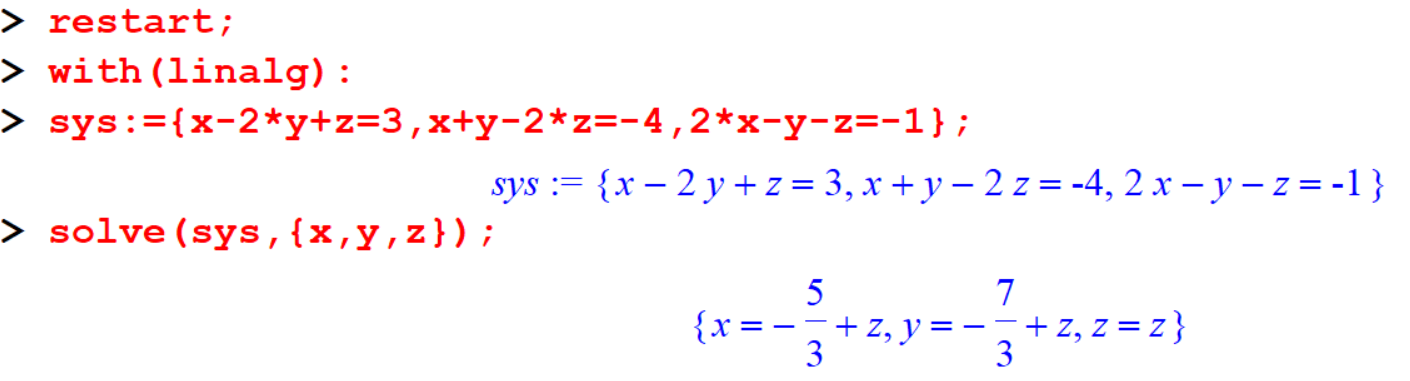
\includegraphics{figures/Lesson 5/fig9.png}

\begin{verbatim}
[> A:=genmatrix(sys,[x,y,z],b);
[> evalm(b);
[> linsolve(A,b);
\end{verbatim}

\emph{output}:

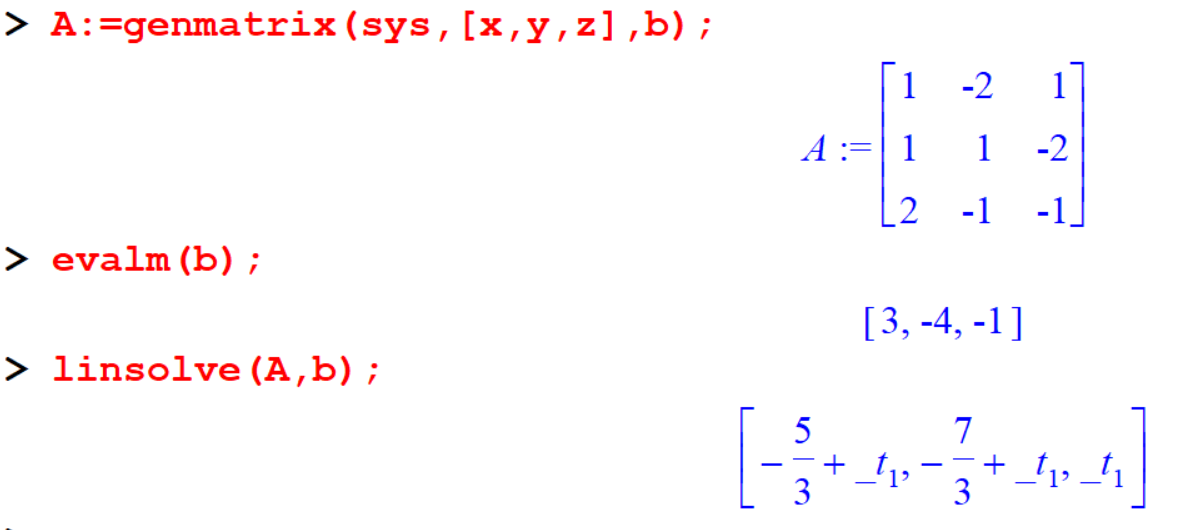
\includegraphics{figures/Lesson 5/fig10.png}

In both cases, the solution contains a parameter.
The \texttt{solve} command express it in terms actual variable used,and the \texttt{linsolve} command use the funny t character to distinguish it from a variable you might have defined yourself.

\begin{center}\rule{0.5\linewidth}{0.5pt}\end{center}

\section{Inconsistent System}\label{inconsistent-system}

An Inconsistent system has no solution. Maple generally, refers to answer questions which have no answer.

\begin{example}
\protect\hypertarget{exm:unnamed-chunk-7}{}\label{exm:unnamed-chunk-7}\[
\begin{array}{ccccccccc}
x &+& y &-& 3z &= 10\\
x &+& y &-&  z &= 1\\
x &+& y &+&  z &= 8  
\end{array}
\]
\end{example}

Let's try to solve this system.

\begin{verbatim}
[> restart;
[> with(linalg):
[> sys:={x+y-3*z=10,x+y-z=1,x+y+z=8};
[> solve(sys,{x,y,z});
\end{verbatim}

\emph{Output}:

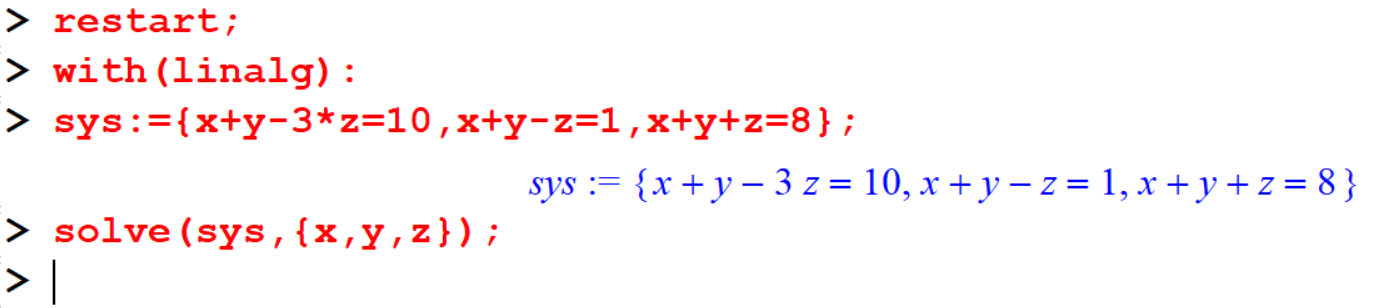
\includegraphics{figures/Lesson 5/fig11.png}

This method does not work. It does not return anything.

Let's try \texttt{linsolve} method.

\begin{verbatim}
[> A:=genmatrix(sys,[x,y,z],b);
[> linsolve(A,b);
\end{verbatim}

\emph{Output}:

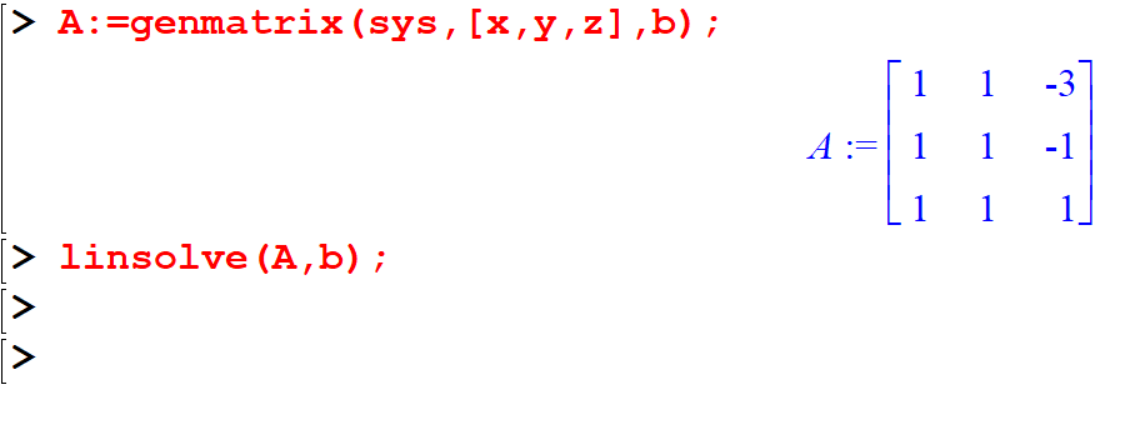
\includegraphics{figures/Lesson 5/fig12.png}

This method also does not works.

\begin{verbatim}
[> evalm(inverse(A)&*b);
\end{verbatim}

\emph{Output}:

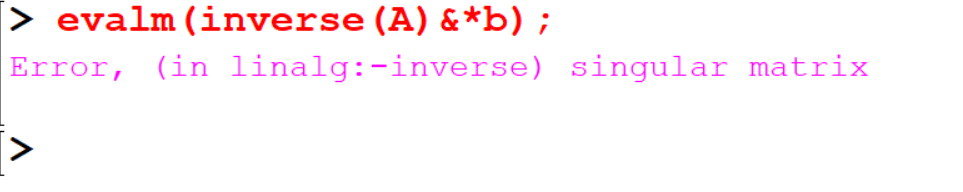
\includegraphics{figures/Lesson 5/fig13.png}

\subsubsection{Automatic Reduction}\label{automatic-reduction}

\begin{verbatim}
[> sys:={3*x+5*y+2*z=12,2*x+5*y-4*z=9,4*x-y+5*z=-3};
[> evalm(b);
[> C:=augment(A,b);
\end{verbatim}

\emph{Output}:

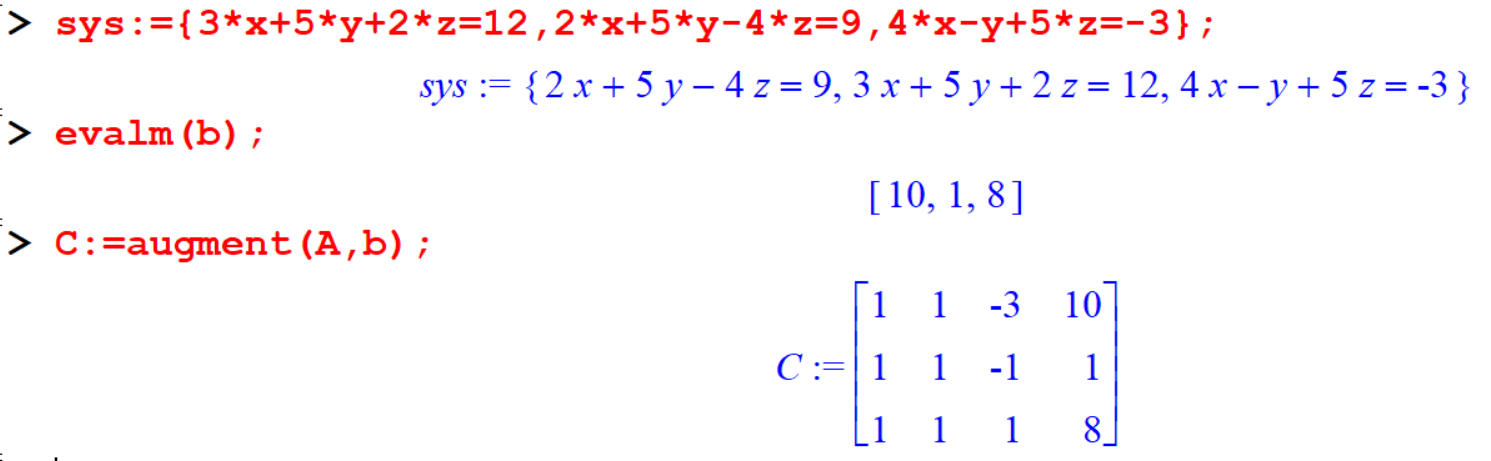
\includegraphics{figures/Lesson 5/fig14.png}

\subsection{Method IV}\label{method-iv}

An even faster method is simplifying let maple to do all the work for us. The \texttt{gausselim} command will perform all of the steps of Gaussian eliminations and reduce an augmented matrix to \textbf{row echelon form}.

\begin{verbatim}
[> sys:={3*x+5*y-2*z=12,2*x+5*y-4*z=9,4*x-y+5*z=-3};
[> A:=genmatrix(sys,[x,y,z],b);
[> evalm(b);
[> C:=augment(A,b);
[> gausselim(C);
\end{verbatim}

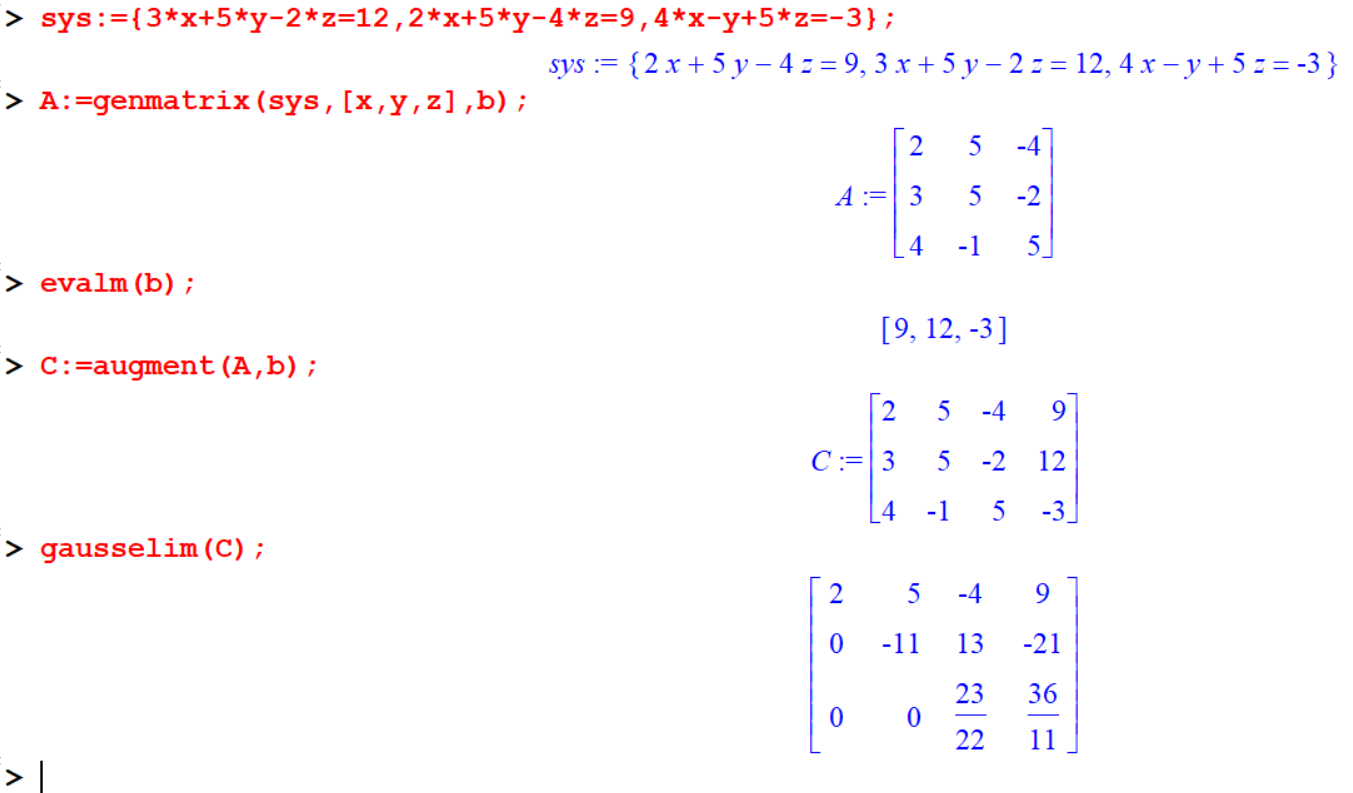
\includegraphics{figures/Lesson 5/fig15.png}

\subsection{Method V}\label{method-v}

The command \texttt{gaussjord} does the same thing.
It performs all the steps of Gauss Jordan elimination and reduces and reduces an augmented matrix into reduced row echelon form.

\begin{verbatim}
[> gaussjord(C);
\end{verbatim}

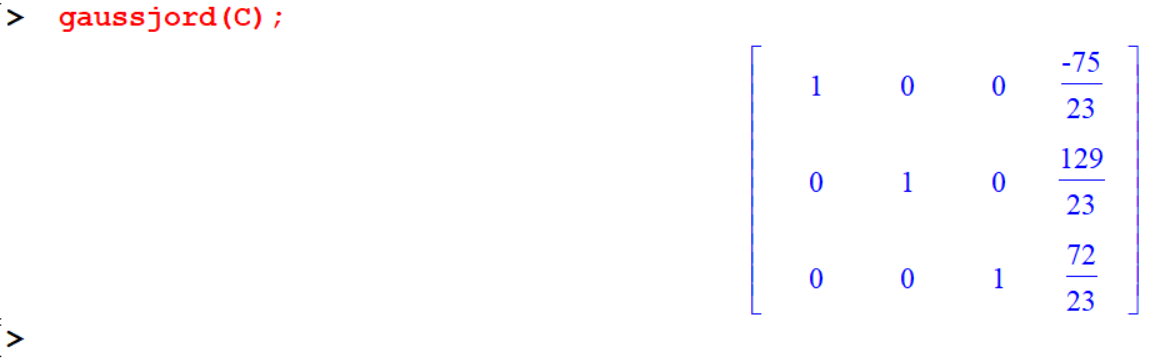
\includegraphics{figures/Lesson 5/fig16.png}

\begin{center}\rule{0.5\linewidth}{0.5pt}\end{center}

\section{Exercise}\label{exercise-1}

\begin{exercise}
\protect\hypertarget{exr:unnamed-chunk-8}{}\label{exr:unnamed-chunk-8}Solve the following system of equations.
\[
\begin{array}{ccccccc}
x_1  &+& 2x_2 &+& 3x_3 &= 9 \\
2x_1 &-& x_2  &+& x_3  &= 8 \\
3x_1 & &      &-& x_3&= 3
\end{array}
\]
\end{exercise}

\begin{exercise}
\protect\hypertarget{exr:unnamed-chunk-9}{}\label{exr:unnamed-chunk-9}

A small manufacturing plant makes three types of inflatable boats: one-person, two-person, and four-person models.
Each boat requires the services of three departments, as listed in the table.
The cutting, assembly, and packaging departments have available a maximum of 380, 330, and 120 labor hours per week, respectively.

\begin{longtable}[]{@{}
  >{\centering\arraybackslash}p{(\columnwidth - 6\tabcolsep) * \real{0.2464}}
  >{\centering\arraybackslash}p{(\columnwidth - 6\tabcolsep) * \real{0.2464}}
  >{\centering\arraybackslash}p{(\columnwidth - 6\tabcolsep) * \real{0.2464}}
  >{\centering\arraybackslash}p{(\columnwidth - 6\tabcolsep) * \real{0.2609}}@{}}
\toprule\noalign{}
\begin{minipage}[b]{\linewidth}\centering
Department
\end{minipage} & \begin{minipage}[b]{\linewidth}\centering
One Person Boat
\end{minipage} & \begin{minipage}[b]{\linewidth}\centering
Two-Person Boat
\end{minipage} & \begin{minipage}[b]{\linewidth}\centering
Four-Person Boat
\end{minipage} \\
\midrule\noalign{}
\endhead
\bottomrule\noalign{}
\endlastfoot
Cutting & 0.5 hr & 1.0 hr & 1.5 hr \\
Assembling & 0.6 hr & 0.9 hr & 1.2 hr \\
Packaging & 0.2 hr & 0.3 hr & 0.5 hr \\
\end{longtable}

\begin{enumerate}
\def\labelenumi{(\Alph{enumi})}
\tightlist
\item
  How many boats of each type must be produced each week for the plant to operate at full capacity?
\item
  How is the production schedule in part A affected if the packaging department is no longer used?
\item
  How is the production schedule in part A affected if the four-person boat is no longer produced?
\end{enumerate}

\end{exercise}

  \bibliography{book.bib,packages.bib}

\end{document}
